\documentclass[a4paper, 11pt]{article}

\usepackage[british]{babel}
\usepackage[autostyle]{csquotes}
\usepackage[colorlinks=true, urlcolor=blue, citecolor=blue]{hyperref}
\usepackage{graphicx}
\usepackage{float}
\usepackage{geometry}
\usepackage[ruled,vlined]{algorithm2e}

\graphicspath{{images/}}
\geometry{margin=2.0cm}

\begin{document}

\title{Borůvka's Algorithm}
\author{Student Number: 690065435}
\date{December 2022}

\maketitle

\begin{abstract}
The minimum spanning tree problem is a fundamental problem in graph theory that has many applications in the real world. In this report, we explore Borůvka's algorithm -- a greedy algorithm that finds a minimum spanning tree for a connected, edge-weighted, undirected graph. We discuss the algorithm's principles, pseudocode, time and space complexity analysis, and applications. We compare Borůvka's algorithm to other minimum spanning tree algorithms such as Prim's and Kruskal's algorithms. We also review variants of Borůvka's algorithm and their use as a two-approximation for the travelling salesperson problem, parallel computation of minimum spanning trees, and faster sequential algorithms for minimum spanning trees.

\begin{center}
\end{center}
\end{abstract}

\vspace*{\fill}
\begin{center}
% TODO: Add link here.
YouTube Video Link:

\vspace{0.5em}
% TODO: Update word count at the end.
Word Count: 1,475

\vspace{1em}
I certify that all material in this report which is not my own work has been identified.
\end{center}
\vspace{1em}

Signature: \hrulefill

\newpage
\section{Principles of Borůvka's Algorithm}
Borůvka's algorithm is a greedy algorithm that finds a minimum spanning tree for a connected, edge-weighted, undirected graph. A minimum spanning tree is a subset of the edges that connects all the vertices without any cycles and with the minimum possible total edge weight \cite{graham1985history}. The algorithm originated from Otakar Borůvka in 1926 as a method of constructing an efficient electricity network for Moravia, a region of the Czech Republic \cite{nevsetvril2001otakar}. Later, it was independently rediscovered by numerous other researchers, most notably by Georges Sollin in 1965, which has led to the algorithm also being known as Sollin's algorithm in parallel computing literature \cite{sollin1965trace}. 

The algorithm is based on the idea of building a forest of trees and uses a hybrid of Prim's and Kruskal's algorithms to find a minimum spanning tree. An advantage of Borůvka's algorithm over Prim's and Kruskal's algorithms is that it does not have to pre-sort the edges, nor does it have to maintain a priority queue. In each iteration, it finds the cheapest edges that connect different trees and uses them to combine trees. Borůvka's algorithm continues to iterate until there is only one tree left -- the minimum spanning tree.

When Borůvka's algorithm was originally discovered, computers did not exist, so the algorithm was implemented by hand -- this explains why the algorithm is simpler and uses basic data structures compared to other minimum spanning tree algorithms such as Prim's and Kruskal's algorithms that were later discovered. Borůvka's algorithm was the first to solve the minimum spanning tree problem in polynomial time \cite{deterministicMSTs}, which was significant because it made it practical to solve the problem for large graphs and therefore more applicable to real-world problems. 

\begin{figure}[h]
    \caption{Borůvka's Short Paper \cite{nevsetvril2001otakar}}
    \begin{center}
        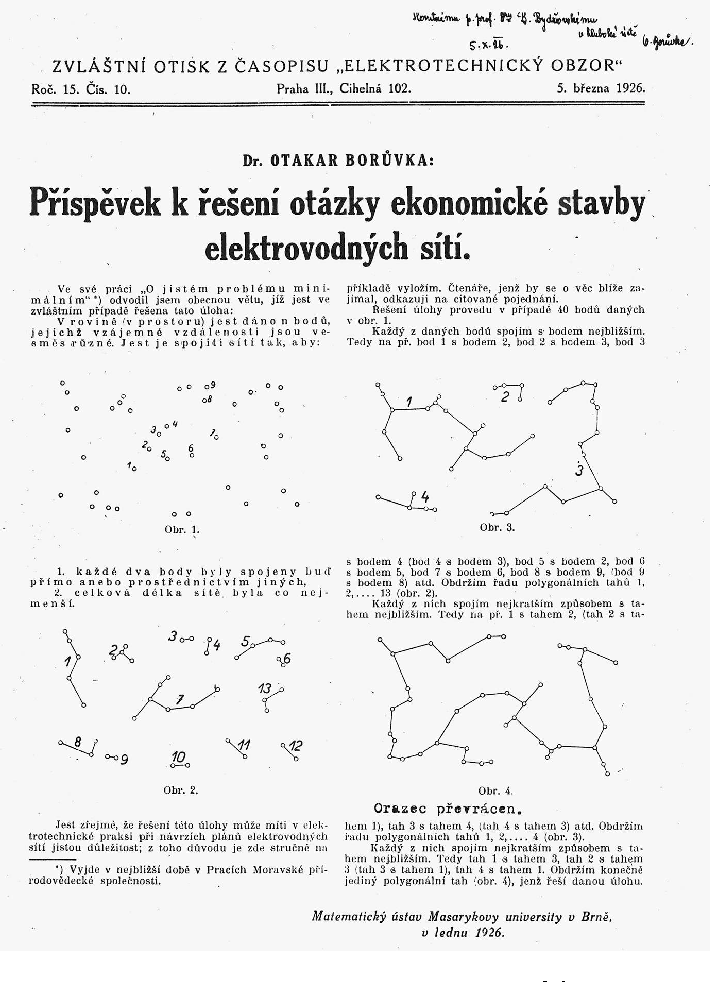
\includegraphics[width=0.55\textwidth]{Boruvka's Short Paper.png}
    \end{center}
\end{figure}

\section{Pseudocode}

% TODO: Revisit this to check whether it's correct and compare it with Python code.
\begin{algorithm}
    \caption{Borůvka's Algorithm}
    \SetKwInOut{Input}{Input}
    \SetKwInOut{Output}{Output}
    
    \Input{A connected, edge-weighted, undirected graph $G = (V, E)$, where V is a list of vertices in the graph, and E is a list of edges in the graph}
    \Output{$T$ (a minimum spanning tree of $G$) and $totalCost$ (the total cost of $T$)}

    \nl Initialise a minimum spanning tree $T$ = (V, E'), where E' = \{\}.

    \nl Initialise the total cost of the minimum spanning tree, $totalCost = 0$.

    \nl Initialise a list of components $N$, where $N_k$ denotes the vertices in component $k$.

    \nl \For{vertex $v \in V$}{
        \nl $N_v = v$.
    }

    \nl \While{$|N|$ > 1}{
        \nl Initialise an empty list of minimum weight connecting edges, $L$ = \{\}.

        \nl \For{component $c \in N$}{
            \nl Initialise the cheapest edge $e$, with weight = $\infty$.

            \nl \For{edge $i, j \in c$}{
                \nl \If{$i, j$ contains an endpoint that isn't in $c$ and weight of $i, j$ < $e$}{
                    \nl Set $e$ to $i, j$.
                }
            }

            \nl \If{$e$ is not $\infty$}{
                \nl Add $e$ to $L$.
            }
        }

        \nl \For{edge $e \in L$}{
            \nl \If{$e$ connects two different components}{
                \nl Merge the components $N_i$ and $N_j$ into a single component, $N_k$, such that $N_k = N_i \cup N_j$.

                \nl Add $e$ to $E'$ in $T$.

                \nl Add the edge's weight to the total cost: $totalCost = totalCost + e.weight$
            }
        }
    }

    \nl \Return $T$ and $totalCost$.
\end{algorithm}

\subsection{Flowchart}
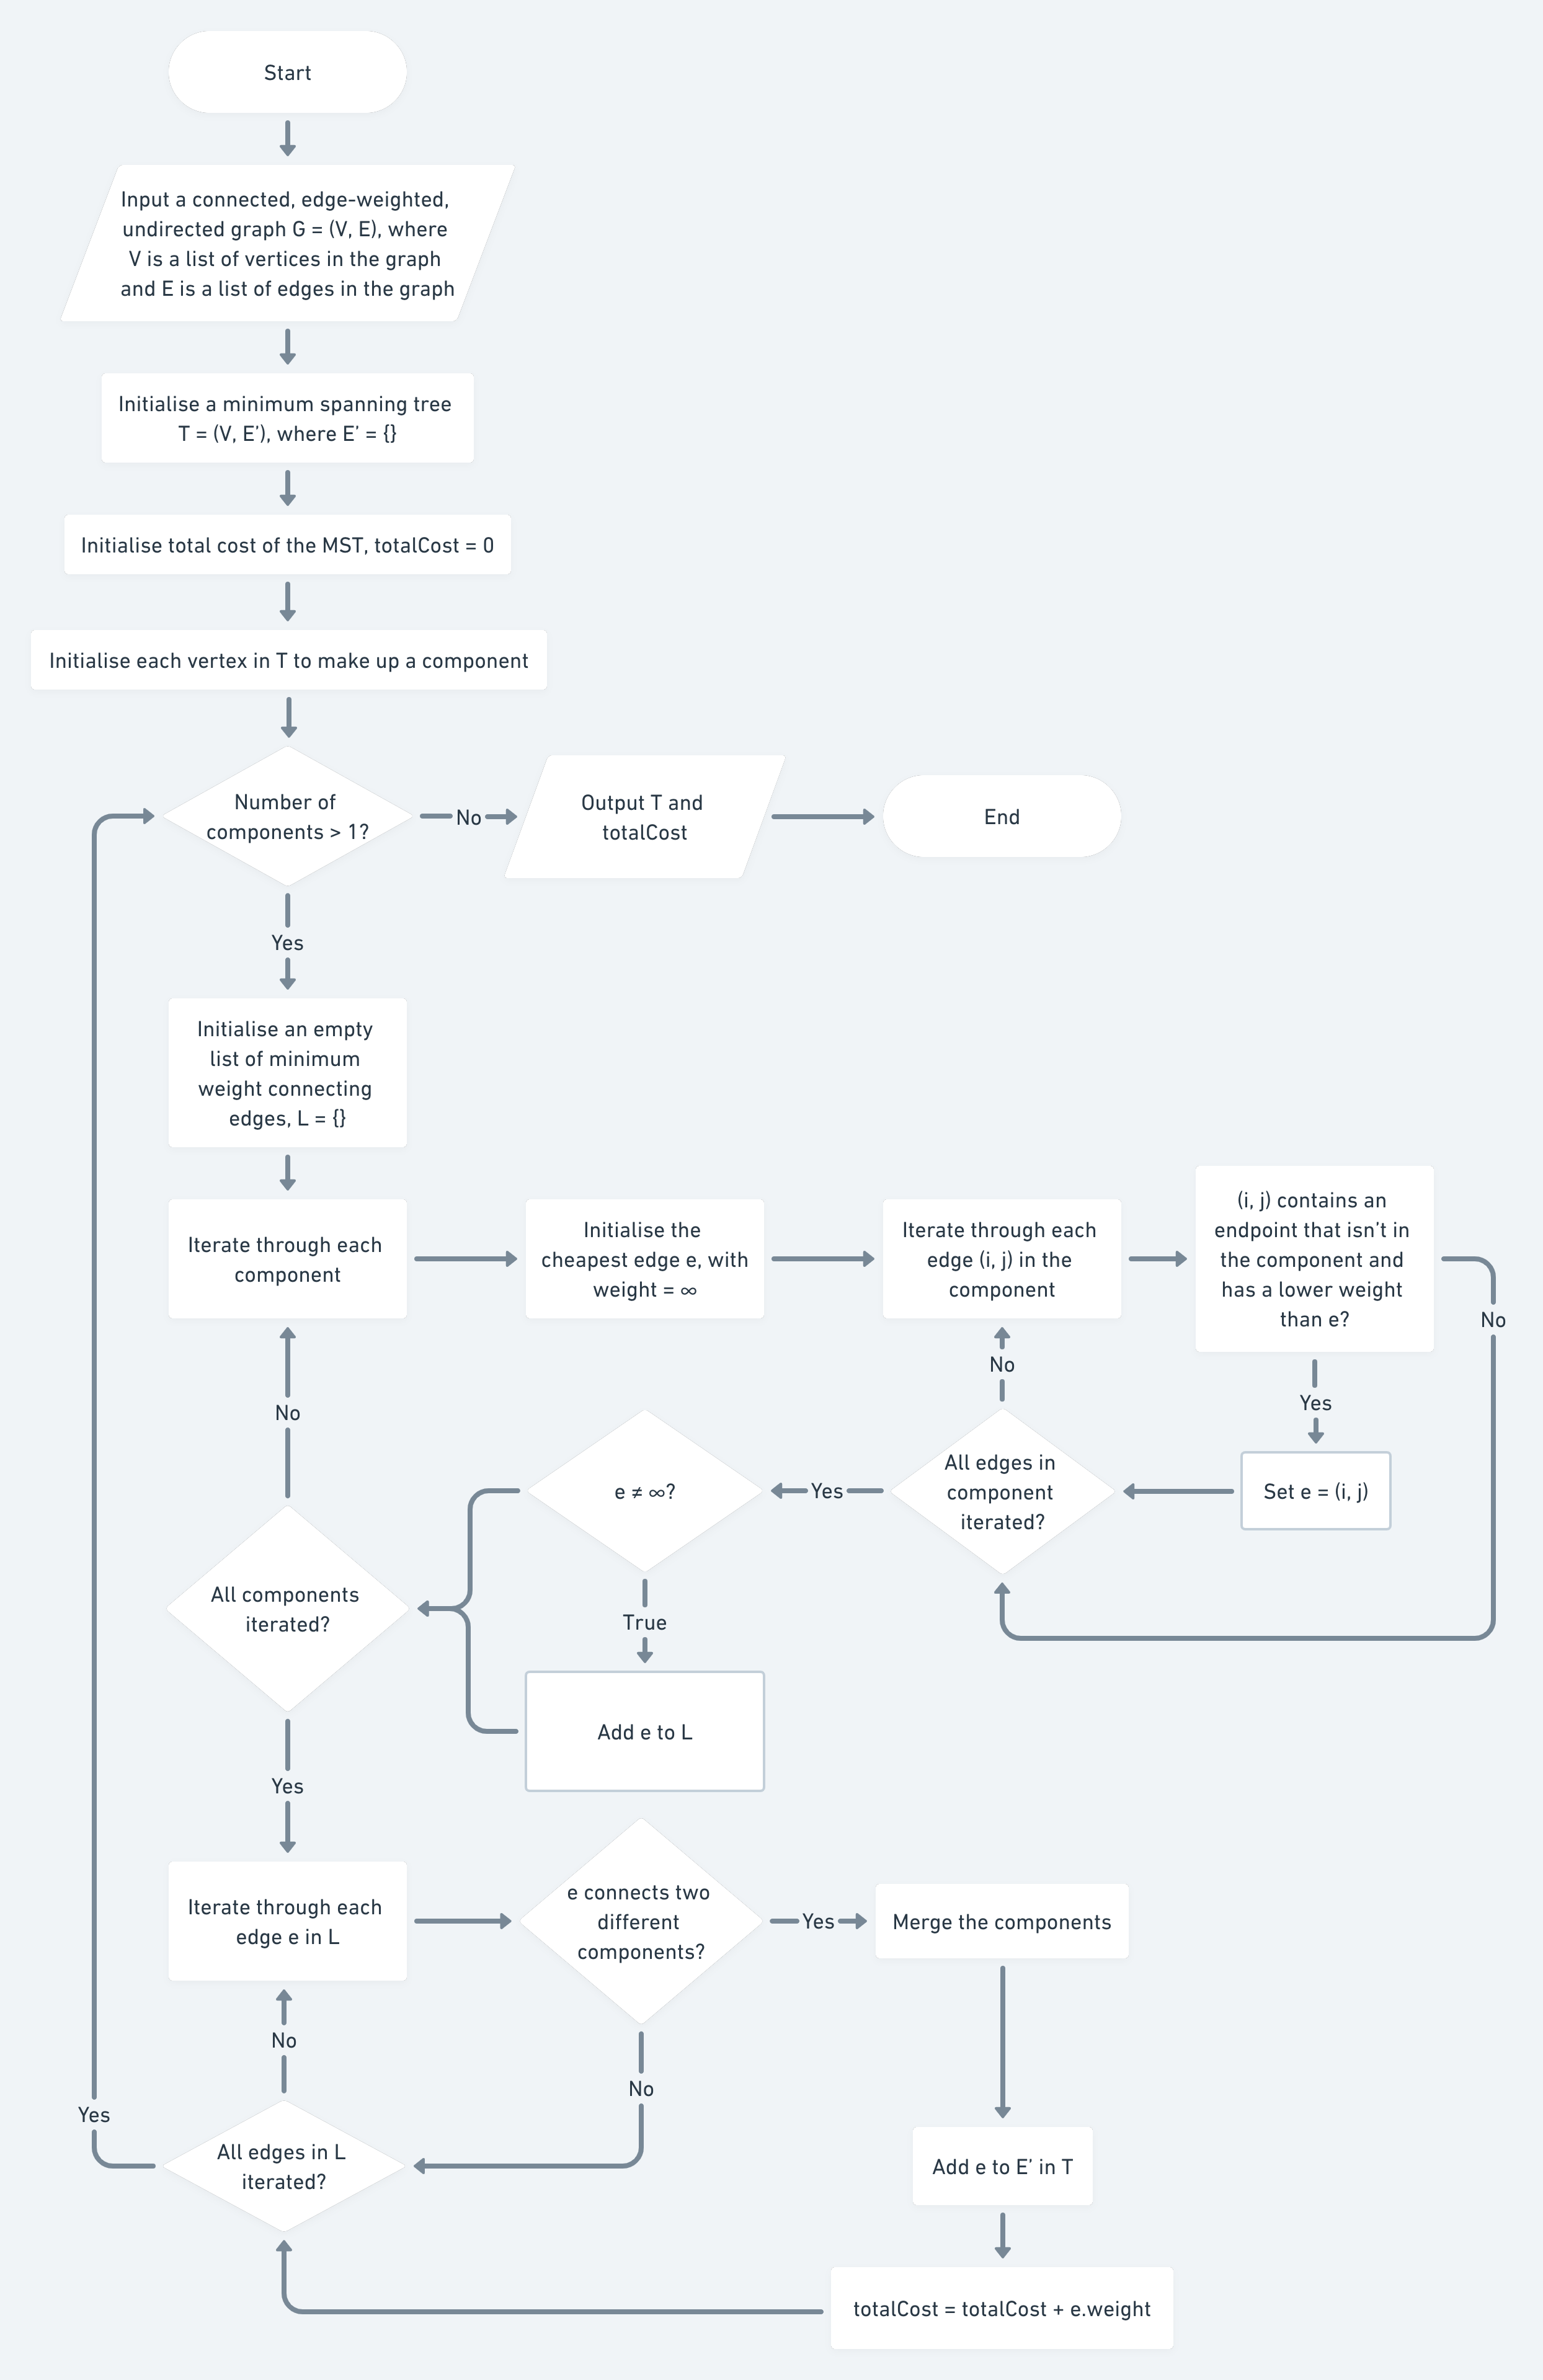
\includegraphics[width=0.95\textwidth]{Flowchart of Boruvka's Algorithm.png}

\section{Time and Space Complexity Analysis}

\subsection{Time Complexity}
\begin{figure}[h]
    \caption{Summary of Borůvka's Algorithm \cite{erickson2014MSTs}}
    \begin{center}
        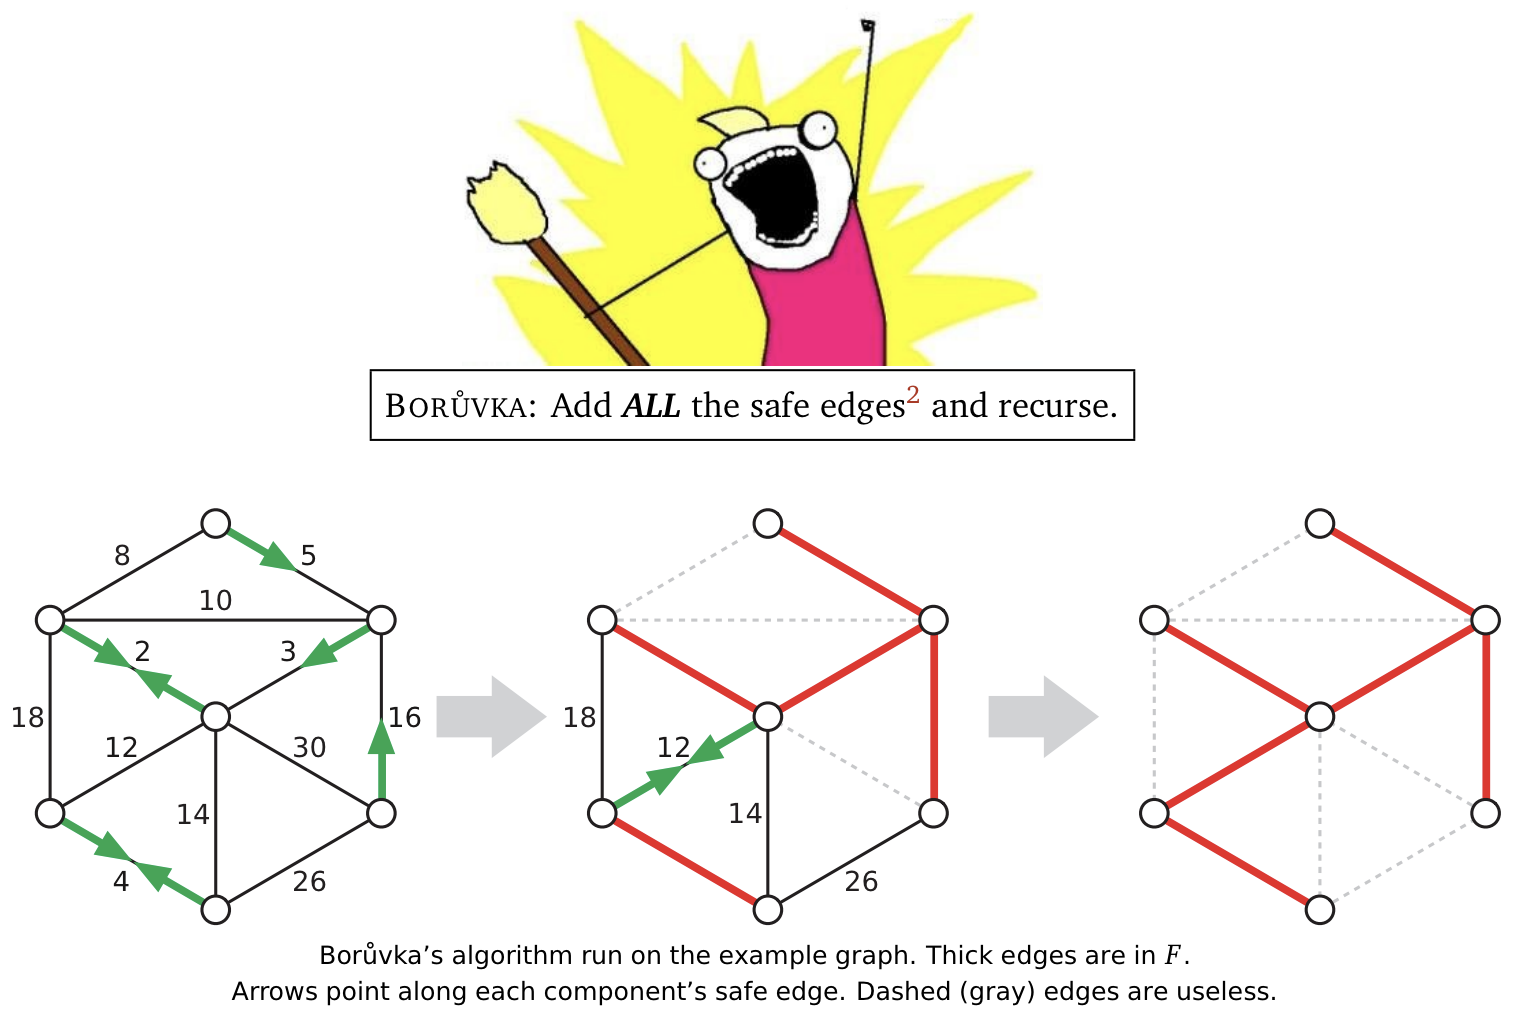
\includegraphics[width=0.8\textwidth]{Summary of Boruvka's Algorithm.png}
    \end{center}
\end{figure}

Borůvka's algorithm has a time complexity of O(E log(V)), where E is the number of edges and V is the number of vertices in the graph.

The outer loop runs for log(V) iterations, as each iteration reduces the number of components by at least a factor of two by combining them -- the worst case occurs when the components coalesce in pairs \cite{erickson2014MSTs}. Within each iteration, the algorithm initialises an empty list of minimum weight edges that connect two components. For each component, it iterates over the edges and updates the minimum weight edge that connects to another component -- this is executed in O(E) time, as the algorithm must consider each edge once. The algorithm then performs a single pass over the minimum weight connecting edges to merge two components into one where possible, which is also performed in O(E) time because each edge can be a minimum connecting edge. This gives a total time complexity of O(E log(V)).

However, Borůvka's algorithm often runs faster than the worst-case runtime of O(E log(V)), as this assumes that the number of components only reduces by a factor of two in each iteration \cite{erickson2014MSTs}. For many graphs, the number of components reduces by a factor of more than two in each iteration, which improves the runtime of the algorithm significantly. The algorithm runs in O(E) time for a broad class of graphs such as planar graphs \cite{cheriton1976finding}, which are graphs that can be drawn on a plane without any edges crossing each other. It does so by removing all but the cheapest edge between each pair of components \cite{marevs2002two}. In contrast, the time analysis for Prim's and Kruskal's algorithms applies to all graphs -- this means that Borůvka's algorithm is more efficient for planar graphs amongst others.

\subsection{Space Complexity}
The space complexity of Borůvka's algorithm is O(E + V), as we must keep a list of components that equates to the number of vertices at the start and a list of minimum weight connecting edges. Prim's and Kruskal's algorithms also have the same space complexity of O(E + V).

\section{Limitations and Constraints}

\subsection{Worst-Case Time Complexity}
Borůvka's algorithm can be slow to find the minimum spanning tree when the graph has a large number of components or when the components in the graph are large. This is because Borůvka's algorithm only considers the cheapest edge that connects two different components, and does not consider the cheapest edge that connects two components that are already connected. Other algorithms such as Kruskal's algorithm and Prim's algorithm do not have this limitation, as they consider all edges in the graph. In the worst case of Borůvka's algorithm, components will coalesce in pairs, and the number of components only reduces by a factor of two -- this means the algorithm must perform more iterations, up to O(log V). 

Compared to Prim's algorithm, which runs in O(E + V log(V)) amortised time when using a Fibonacci heap \cite{fredman1987fibonacci}, Borůvka's algorithm is slightly slower in worst-case scenarios. However, this variation of Prim's algorithm with the Fibonacci heap is more complicated to implement, and there are many types of graphs that Borůvka is more efficient at solving, such as planar graphs. In the next section, we will also explore parallelisation with Borůvka's algorithm, which is not possible with Prim's. Based on these factors, Borůvka's algorithm is generally more efficient than Prim's algorithm in practice.

\subsection{Directed Minimum Spanning Tree Problem}
Borůvka's algorithm only works on undirected graphs as it does not account for the direction of the edges. Thus, it cannot solve the directed minimum spanning tree problem, which is more complex than the minimum spanning tree problem. Other algorithms such as the Chu-Liu/Edmonds' algorithm (originally proposed in 1965) can solve the directed minimum spanning tree problem \cite{gabow1986efficient}.

\section{Applications}

\subsection{Designing Networks in the Real World}
As Borůvka's algorithm finds a minimum spanning tree, it is most directly used in the design of networks, such as electrical networks, communication networks, and transportation networks \cite{graham1985history}. In the original application of an electricity network for Moravia, the vertices represented towns, and the edges represented the distances between towns. Borůvka used the assumption that it was not necessary to directly connect every town to the source of electricity -- it was sufficient for a town to connect via another town that was already connected to power \cite{nevsetvril2001otakar}.

\subsection{Two-Approximation for the Travelling Salesperson Problem}
Borůvka's algorithm satisfies the triangle inequality and finds a minimum spanning tree, so it also acts as a two-approximation algorithm for the travelling salesperson problem \cite{andreae1995performance}, which is NP-hard and thus not possible to solve in polynomial time \cite{junger1995traveling}. Because it produces a two-approximation, the output is at most twice the cost of the optimal solution. This can be proven as the total cost of a full walk is at most twice the cost of the minimum spanning tree, and the algorithm returns a path with a cost less than the full walk, as our pre-order walk replaces two or more edges of the full walk with a single edge \cite{andreae1995performance}.

\begin{algorithm}
    \caption{Two-Approximation for the Travelling Salesperson Problem with MST-DFS \cite{andreae1995performance}}
    \nl Set a vertex as the start.
    
    \nl Construct a minimum spanning tree, $T$.
    
    \nl Create a list of vertices, $H$, that is ordered according to when they are visited in a pre-order tree walk of $T$, and add the start vertex at the end.
    
    \nl Return the path $H$.
\end{algorithm}

\newpage
\subsection{Parallel Computation of Minimum Spanning Trees}
Several other algorithms are technically more optimal for finding a minimum spanning tree depending on the input graph -- Prim's algorithm is faster for dense graphs, and Kruskal's algorithm is faster for sparse graphs \cite{bazlamaccci2001minimum}. However, this only considers sequential implementations of the algorithms -- Borůvka's algorithm has become increasingly popular because it is easy to parallelise \cite{mariano2015generic}. This contrasts with the aforementioned algorithms, which are intrinsically serial -- they start with a single component and seek to add edges to it, making it difficult to parallelise them as we must keep and check edges in a strict order. As Borůvka's algorithm starts with multiple components and seeks to connect them with the shortest edge, it can be parallelised by distributing the edges between processors to determine the shortest connecting edge for each vertex \cite{chung1996parallel}. The parallel implementation of Borůvka's algorithm enables faster performance on multi-core or distributed systems, giving it an advantage over other classical minimum spanning tree problems when working at a large scale.

\subsection{Faster Sequential Algorithms for Minimum Spanning Trees}
The concepts behind Borůvka's algorithm have also been used to develop faster sequential algorithms. For example, the expected linear time minimum spanning tree algorithm proposed by Karger, Klein, and Tarjan runs in O(E) time. It involves an adaptation of Borůvka's algorithm by using the Borůvka step, which reduces the number of vertices in the graph by at least a factor of two, on graph G to create a contracted graph G' \cite{dixon1992verification, king1995simpler}. This is followed by a random sampling step that selects a subgraph H by selecting each edge in G' independently with a probability of 1/2 \cite{bazlamaccci2001minimum}. Finally, the verification step removes F-heavy edges from G' to reduce the graph further using a linear time minimum spanning tree verification algorithm \cite{dixon1992verification, king1995simpler, karger1995randomized}.

\newpage
\bibliography{main}
\bibliographystyle{ieeetr.bst}

\end{document}